\documentclass{article}
\usepackage{minted}
\usepackage{graphicx}
\usepackage{calligra}


\author{Manuel Flückiger 22-112-502}
\title{Rechnerarchitektur Serie 4}
\date{\today}

\begin{document}

\newcommand{\mycomment}[1]{}

\maketitle

\section*{Theoretical Questions}
\section{Sign Extension \_/1 Point}
Explain why the sign extension is especially needed for branch-, load- and store-instructions. \newline
All I-format instructions, such as loads, stores, and branches, need sign extension. The bits that 
are extended are the address field bits (the instruction’s least significant 16 bits). 
The sign extension’s output will be an input for some kind of adder, which requires two 
32-bit values as input. We can use a negative offset from the register value for loads and stores. 
For example, when accessing local values from a stack pointer, negative offsets are often used. 
Backward branches, like the ones in loops, need a negative offset from the program counter.
\section{Logical and Bitwise Operations in C \_/1 Point}
Determine the corresponding outputs:\newline
\begin{tabular}{|c|c|c|}
    \hline
    Operation & Result & Explanation\\
    \hline
    0x0 \&\& 0xEF & false & \&\& returns 1 (true) if both values are non-zero, 0x0 = 0, 0xEF = 239 \\
    \hline
    0xD3 \& 0x5B & 0x53 & bitwise and operator: 11010011\& 01011011 = 01010011\\
    \hline
    0x0 \textbar\ \textbar\ 0xEF & 1 & returns 1 (true) if either values are non-zero\\
    \hline
    0xA3 \textbar\ 0x3A & 0xBB & bitwise or operator: 10100011 \textbar 00111010 = 10111011\\
    \hline
    !0xFE & false & 0xFE = 254 = true. With the logical NOT infront, this changes to 0\\
    \hline
    $\sim$0xFE & 0x01 &  bitwise not inverts all bits ∼11111110 \rightarrow 000000001 \rightarrow 0x01\\
    \hline
    \end{tabular}

\section{infinite Loop \_/2 points}
The programmer intended the following MIPS program to execute foo in line 8 exactly nine times.
However, the program does not terminate. Explain why and fix the problem while preserving the
original intent (reordering, modifying or removing instructions is not allowed).\newline
The reason for this is that the code does not update the return address (\$ra) register when 
calling the foo subroutine on line 4. The \$ra register holds the address of the instruction 
to return to after a subroutine call. In this case, the \$ra register should be set to line 5, 
but it is not. Therefore, when the foo subroutine executes the jr \$ra instruction on line 11, 
it jumps back to line 4 instead of line 5, and repeats the loop indefinitely.

To fix this problem, you need to use the jalr instruction instead of jal on line 4. The jalr 
instruction jumps to a subroutine and sets the \$ra register to the address of the next 
instruction. This way, when the foo subroutine returns, it will resume from line 5 and 
decrement the loop counter (\$t0) as intended.

\section{bne instead of beq \_/2 Points}
What changes are needed in the MIPS implementation presented in the lecture (see slide 16 “003-
Einführung in MIPS.pdf”) to implement bne instead of beq?\newline
\textit{weird reference.}
\begin{itemize}
\item[(a)] For the singlecycle implementation \newline
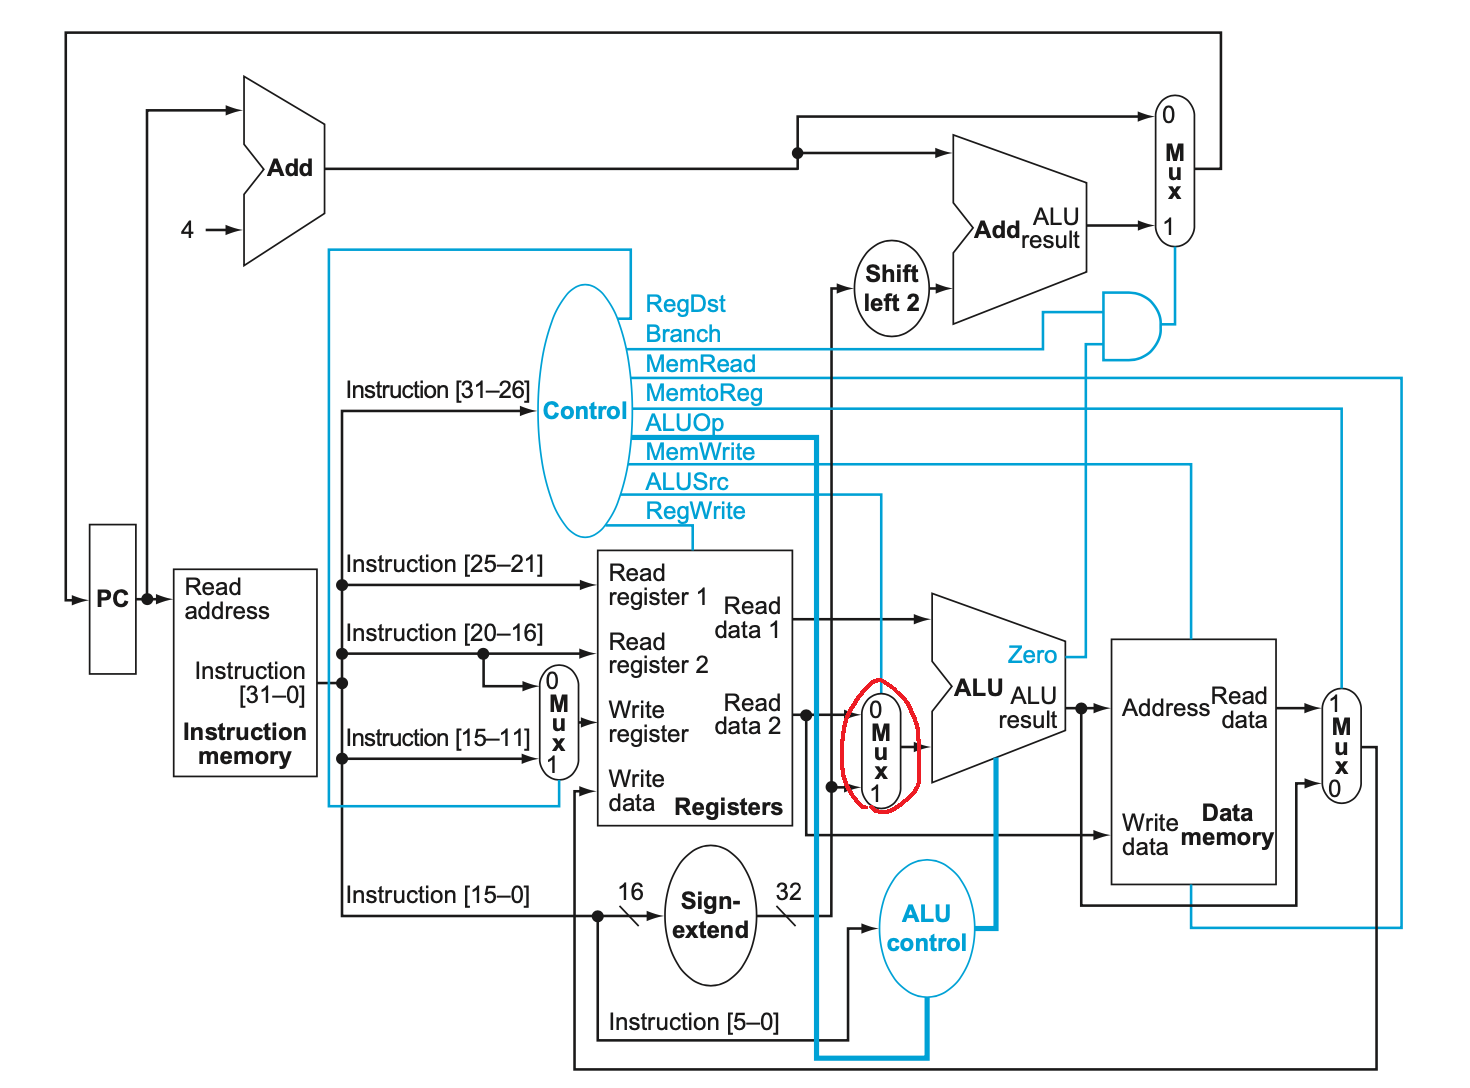
\includegraphics[width=\textwidth]{mipssinglecyclemarked.png}
The, in red marked, multiplexer should be inverted, so 1 is up and 0 is down.

\item[(b)] For the multicycle implementation. \newline
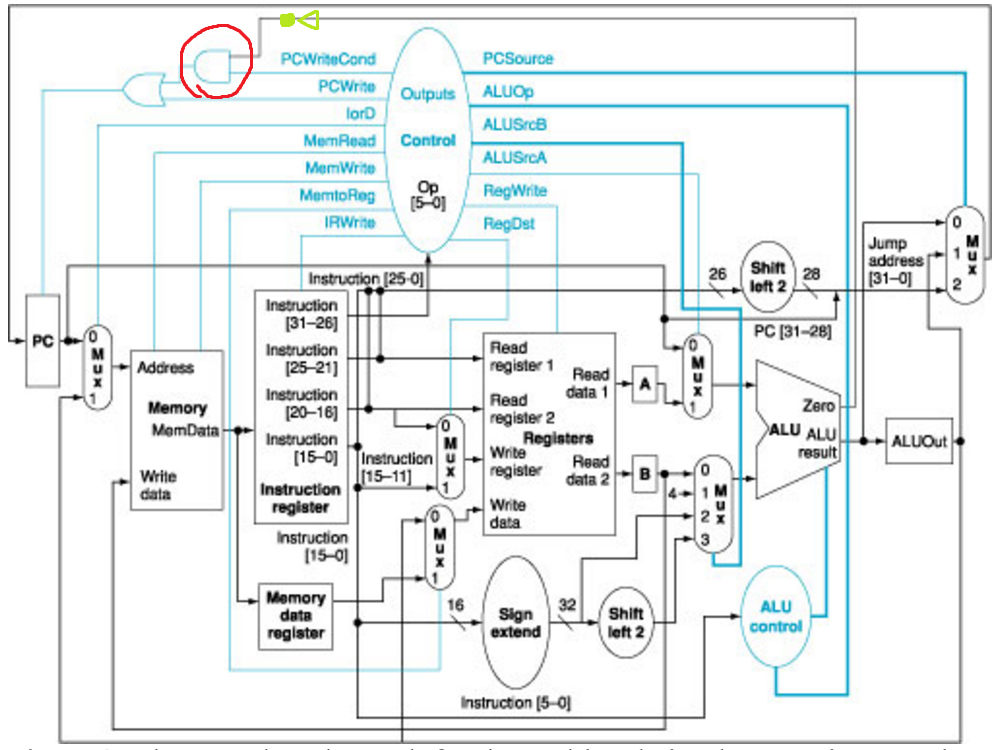
\includegraphics[width=\textwidth]{multycyclemarked.png}

The, in green added, NOG must be added before the logical AND.

\end{itemize}


\section{Pipeline Registers \_/1 Points}
What are the registers (see slide 8, “005d-Der-Prozessor - Pipeline.pdf”) between the states needed
for?
The values need to be stored temporarily, otherwise they would be overwritten in the next step or the 
previous step would alter the output too quickly.

\section{Pipelining Hazard \_/2 Points}
Explain the difference between control, data and structural hazards.
\begin{itemize}
    \item Control hazards: Caused by delay between the fetching of instructions and decisions about 
    changes in control flow (branches and jumps)
    \item Data hazards: Instruction depends on result of prior instruction still in the pipeline.
    \item Structural hazards: Hardware cannot support certain combinations of instructions 
    (two instructions in the pipeline require the same resource).
\end{itemize}
\section{Stall \_/2 Points}
Explain why on slide 19 it is enough to wait two clock cycles but not on slide 23 (the slide numbers
refer to the chapter “005d-Der-Prozessor - Pipeline.pdf”).\newline
The register in slide 19 can be overwritten and read in the same cycle. Therefore, in contrast 
to slide 23, one cycle can be saved because it cannot be read in the same cycle.
\rightarrow Slide 23 has an extra stall compared to slide 19
\section{Data Hazard \_/2 Points}
Show all data hazards in the following code. Which dependencies are data hazards that can be
resolved by forwarding? Which dependencies are data hazards that will lead to a stall ?
\begin{verbatim}
1 add $t0, $t5, $t4
2 lw $s2, 0($t0)
3 sub $s3, $t0 ,$s2
4 sw $t4, 4($s3)
\end{verbatim}
There are 3 RAW hazards, marked by $_{number}$:\newline
1 add \$t0$_1$, \$t5, \$t4 \newline
2 lw \$s2$_2$, 0(\$t0$_1$) \newline
3 sub \$s3$_3$, \$t0 ,\$s2$_2$ \newline
4 lw \$t4, 4(\$s3$_3$) \newline
Can be solved by: \newline
1: forwarding is enough\newline
2: stall is needed\newline
3: forwarding is enough\newline
\end{document}
